\chapter{Neural networks for the prediction of RI of 1.5 million organic molecules}

 One of the most important and non-trivial properties of these molecules is the molecular packing. The packing density of organic molecules is highly dependent on the molecular structure. Organic molecules with a targeted density can be achieved by controlling the chemical structure. We can understand more about the correlation between the molecular structure and packing density of molecules by studying a large number of molecular candidates. Using our in-house molecular generator, we generated a molecular library of 1.5 million small organic molecules. The most accurate way to evaluate the density of these molecules is by performing molecular dynamics (MD) simulations. Since MD simulations are computationally intensive, performing simulations for a large library of molecular candidates is not a viable option. Therefore, we selected hundred thousand molecules from the library and evaluated their density values. Using this data as training set, we developed an exceedingly efficient ($R^2$=0.98) neural network model to correlate molecular structural descriptors with their properties. Using this correlation, we were able to quickly compute the density values of 1.5 million organic molecules. We mine this huge data to obtain insights into the correlation between the molecular structure and density of materials. Additionally, we evaluate the learning curve for the density prediction to obtain a correlation between the model efficiency and size of the data. We demonstrate that the developed machine learning approach is a powerful tool and has shown to be highly promising for rapidly identifying molecular candidates with a targeted density. 
 


\section{Introduction}
\label{sec:introduction}

The packing of particles in a given volume has garnered the interest of researchers from a variety of disciplines for over a centrury \cite{Kwan2009}. Packing density, directly impacts ionic conductivity \cite{Swenson1996} or mobility in solvents \cite{Shen2015}, optical properties \cite{Ando2006}\cite{Terui2004} and other applications in physical organic chemistry \cite{Sheu1989}. In the current century, there is a pressing demand for discovering new materials with superior mechanical, optical and other bulk properties and a negligible negative impact on the environment. The traditional trial-and-error approach for experimental research has proved to be time consuming and resource intensive. The advent of stable and efficient computational power has paved the way for computational and data-driven research to take the center stage in materials discovery. 

Machine learning has been established as a reliable approach to accelerate prediction of material properties and materials discovery \cite{Olivares-Amaya2011}. The ability to predict the properties of novel materials prior to synthesis, and to understand the relationships between the microscopic properties of molecular components and the macroscopic materials properties, would be of substantial benefit to materials discovery \cite{Hachmann2014}. There is a strong need for machine learning methods that can generate robust, predictive models linking these microscopic properties. Artificial Neural Networks have been widely accepted as an efficient computational model used in machine learning. Multi-layer NNs have been used to predict properties like RI \cite{Alexandridis2012}, dielectric constant \cite{Mannodi-Kanakkithodi2016}, atomization energy \cite{Montavon2012}, chemical reactivity \cite{Simon1993}, melting point \cite{Karthikeyan2005}, viscosity \cite{Gharagheizi2007}, solubility \cite{Huuskonen1998}, etc.

Focusing on the increasing demand for complex and intricate optical appliances, it has become imperative to find easily processable materials with superior optical properties, good mechanical integrity, eco-friendly nature and economically viability. A holistic materials approach has brought to light the viability of organic ‘High Refractive Index Polymers’ (HRIPs) for such optoelectronic devices \cite{Higashihara2015} \cite{Macdonald2014}. Since linear optical properties are directly or indirectly dependent on packing density \cite{Terui2004}, an accurate model for its calculation would play an important role in the computationally driven quest to discover suitable HRIPs. Packing density can be improved by controlling the molecular or chemical structure and an efficient model to calculate it would allow us to tune various properties to develop suitable HRIPs in accordance with their targeted area of use \cite{Tanio1994}.  

The goal is to select suitable candidates from a large library of molecules. For this it is primarily essential to establish a protocol for accurately calculating packing density. For the purpose of benchmarking, three different methods are employed to calculate density of commonly used small organic molecules and the results are compared to their corresponding experimental values. This comparison displays the supremacy of Molecular Dynamics as the most accurate method for density calculation. As the evaluation of density of a large library of molecules is computationally expensive, we develop a NN model to accelerate the density calculation. We perform molecular dynamics simulations within a virtual high-throughput framework to automate the evaluation of density values of a hundred thousand molecules and use the resulting data as the training set for learning the NN model. This enables us to accurately and swiftly predict density values for the larger data set of 1.5 million molecules.

In addition to identifying the best candidates from our high throughput screening studies, we analyze the collected data to further understand structure property relations. The building blocks that contribute the most towards high density values are identified using Z-score analysis. Additionally, the building blocks that are prominent in a particular density interval are also identified using Z-score mapping for the entire density range. 



\section{Methods}
\label{sec:methods}

\subsection{Bondi's Method}
\label{subsec:bondis}

As per Bondi's method, we obtain the van der Waal’s volume ($V{}_{vdw}$) from the contribution of individual atoms \cite{Bondi1964} and assume the packing fraction to be a constant. Applying a correctional factors to the sum of atomic volumes, we use equation II.1 to obtain $V{}_{vdw}$, where $V_i$ is the volume of atom $i$, $N_B$ is the number of bonds, $N_{ar}$ is the number of aromatic rings and $N_{non-ar}$ is the number of non-aromatic rings in the molecule \cite{Zhao2003}. We calculate the molecular volume from $V{}_{vdw}$ by using Slonimskii's method as shown in equation II.2, where $K_p$ is the packing constant of the material \cite{Slonimskii1970}. Once the molecular volume is obtained, we compute the density of the material ($\rho$) by using the equation II.3.

\begin{align}
V{}_{vdw}=\Sigma V_i - 5.92N{}_B - 14.7N{}_{ar} - 3.8N{}_{non-ar}\
\end{align}
\begin{align}
V{}_{mol}=\frac{V{}_{vdw}}{K{}_p}\
\end{align}
\begin{align}
\rho=\frac{M{}_W}{N{}_A V{}_{mol}}\
\end{align}

\subsection{Wavefunction method}
\label{subsec:wavefunction}

Similar to the previous method, the wavefunction approach also calculates the density from the van der Waal's volume using equation II.2 and II.3. The only difference lies in the fact that the van der Waal's volume here is obtained from the wavefunction of molecules using the Monte Carlo technique. We obtain the wavefunction of molecules from quantum calculations using the GAMESS quantum chemistry code \cite{Micheal1993}. In the Multiwfn software we then define a box of volume $L$ that fits the entire system \cite{Lu2012}. Using the Monte Carlo principle we randomly distribute $N$ particles in the box and if $n$ particles are present within the van der Waal's region, then the van der Waal's volume of the system is given by $n/N*L$. 

\subsection{Molecular Dynamics Method}
\label{subsec:mdmethod}

The third method that we use to calculate density, is the Molecular Dynamics method. We use Openbabel to create a file representing the 3D structure of the molecule from their SMILES code. We then pre-optimize molecular structures in the MMFF94s force field using the steepest descent algorithm \cite{OBoyle2011}. We compute the packing density of the molecules using the general amber forcefield (GAFF) \cite{Wang2004}. We use the Antechamber toolkit within AmberTools to generate GAFF parameters for the molecules in an automated fashion \cite{Wang2006a}. Our simulations are carried out using GROMACS (GROningen MAchine for Chemical Simulations) \cite{Beredsen1995}, which is a molecular dynamics package developed by the Biophysical Chemistry department of the University of Groningen. We use the solvate tool within GROMACS to create a simulation box of 10nm and fill it with pre-optimized molecules. The system is first subjected to a minimization step to minimize the internal energy associated with construction of bonds, bond angles and bond dihedrals. This is followed by NVT and NPT equilibration for 100 ps and 240 ps respectively. Both NVT and NPT ensembles use a Nose-Hoover thermostat at 298.15 K for temperature control, while the NPT ensemble uses the Parinello-Rahman barostat for pressure control. We conclude the MD process with a final NPT production run which lasts 40 ps. We compute the final density by averaging out the density values of the system at intervals of 0.2 ps in the production run. 


\subsection{Neural Networks}
\label{subsec:nn}

%The results from the MD simulations were used to train a NN model to predict the density of a large library of molecules. 
We generated the NN model within a feature space of 197 molecular descriptors on a training data set of 100,000 molecules with density values computed using molecular dynamics. Details of the descriptors can be found in the Supplementary Material. For the initial model evaluation, the data set of 100,000 molecules was randomly divided into 80\% training and 20\% test set for testing. 
The NN modeling was performed using \chemml 0.9 \cite{Haghighatlari2017}, our program suite for machine learning and informatics in chemical and materials research. In this work, \textit{ChemML} employed the scikit-learn 0.18.2 multi-layer perceptron (MLP) regressor 1.17.1 \cite{scikit-learn} and descriptors from Dragon 7 \cite{Taletesrl2011}. We applied grid search method to optimize the hyper-parameters of NN model.
The final NN model included two hidden layers having 100 neurons each. 	We constructed the model using rectified linear unit as the activation function, 'adam' solver for weight optimization, adaptive learning rate, and an L2 regularization parameter of 0.0001. 

To evaluate the learning curve, we increased the training set size in increments from 0.5\% to 100\%. For every training set size, we applied bootstrapping method to evaluate the model performance. This method includes randomly selecting the training set from the complete data set and testing on the remaining data set. The process is repeated 50 times by replacing the previous test set, i.e. all the 50 repetitions are independent of each other. The mean and deviation of $R^2$ value from these 50 repetitions for each training size is used for plotting the density learning curve. 
%For every molecule, descriptors were extracted from the Dragon software for use as a feature vector. The total number of features used are 197. The NN was built using a rectified linear unit activation function, Adam solver and an adaptive learning rate. We applied grid search method to optimize the learning parameters of NN model. %The training set had 80,000 density values from the MD calculations and the test set had 20,000 density values from the same.  

\subsection{\chemhtps}
\label{chemhtps}

Controlling density of materials with different functional groups by tailoring the chemical structure is rather difficult. It could potentially lead to an infinite number of candidate molecules. Therefore it is impractical to empirically characterize a large number of candidates. On the other hand, computational analysis allows greater exploration at a fraction of the time and cost. A large candidate library of 1.5 M small organic molecules is generated using our in-house molecular library generator. The library is generated using combinatorial linking of 15 building blocks (see Fig.\ \ref{fig:BB}) for 4 generations, while enforcing constraints like molecular weight within the range of 150 to 400 and setting the maximum number of rings to 4. The complete library can be found in our database (Need an online database)

\begin{figure}[htbp] 
	\centering
	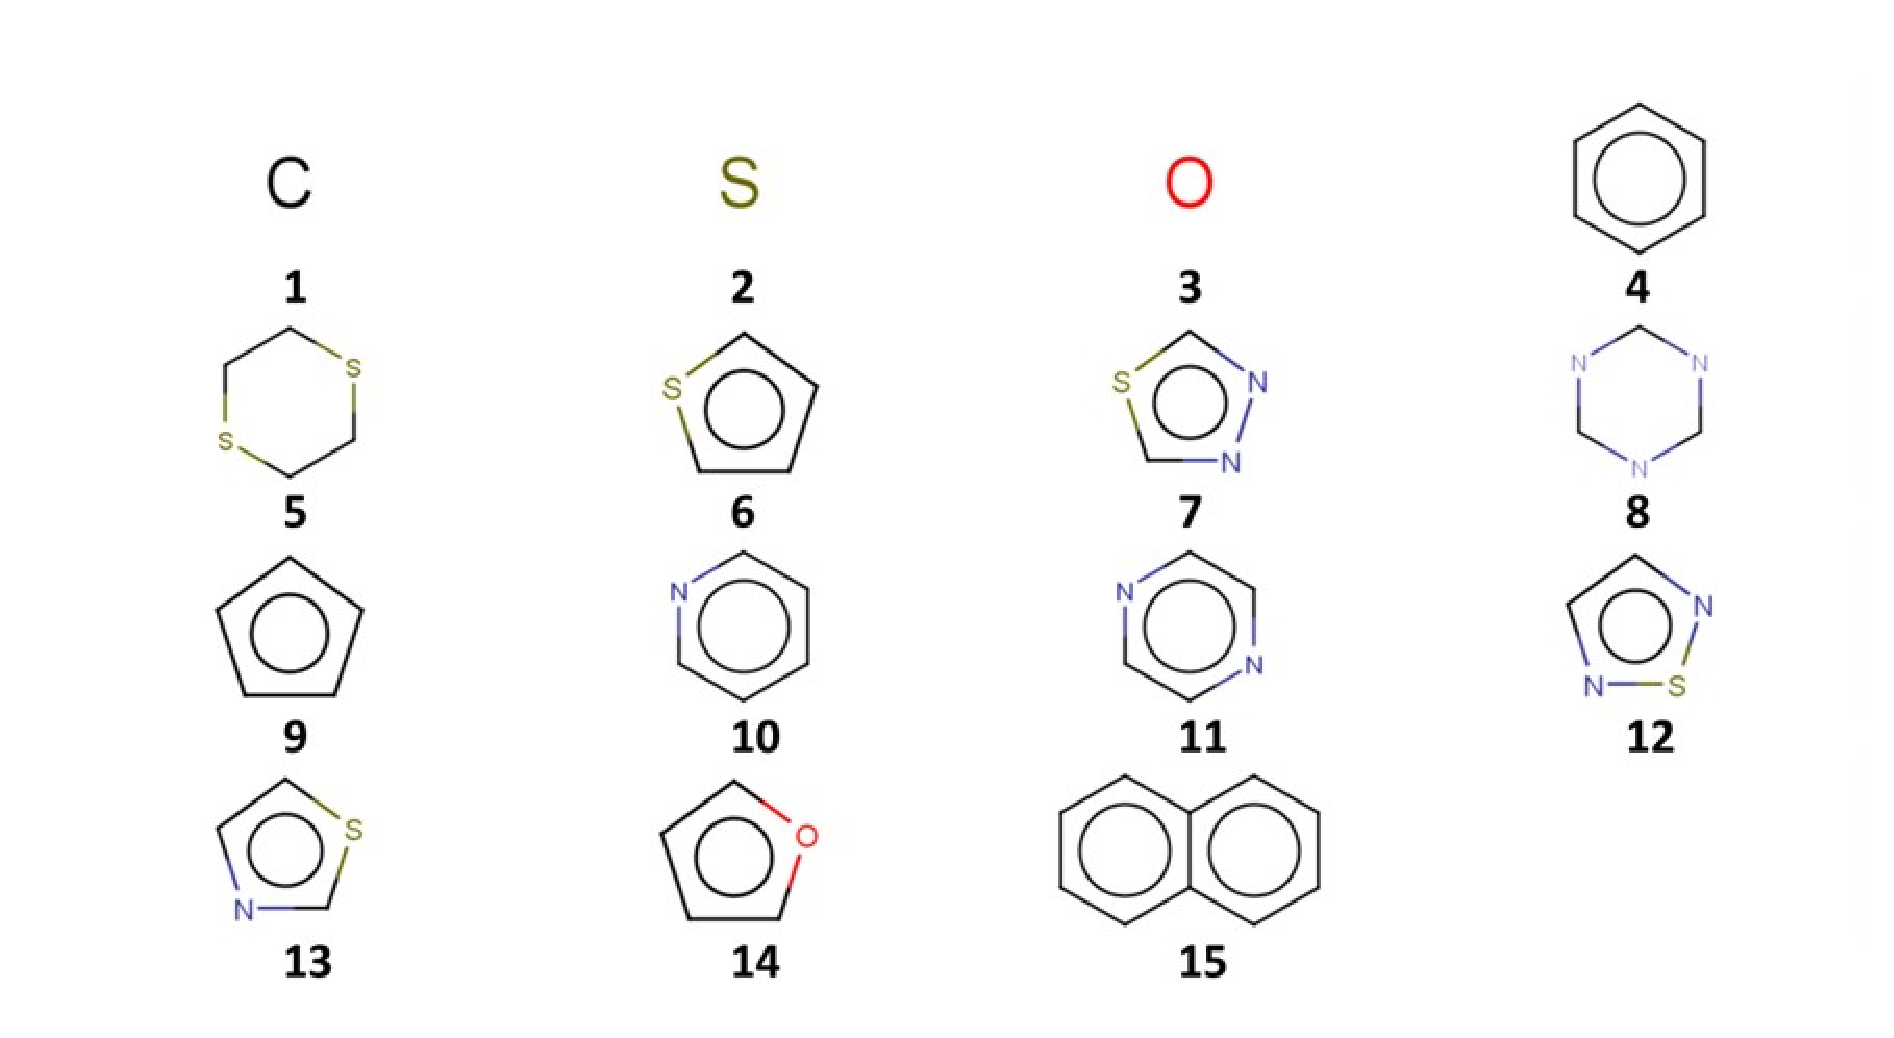
\includegraphics[width=0.744\textwidth]{Chapter-6/Figures/BB_list.eps}
	\caption{Building blocks used to build a library of 1.5 million molecules.}
	\label{fig:BB} 
\end{figure} 

To facilitate density evaluation of the large library that was generated in a timely and efficient way, we use our virtual high throughput screening framework \chemhtps. \chemhtps draws inspiration from the Harvard Clean Energy Project which successfully screened millions of organic molecules for photovoltaic applications. Not only does it create inputs, executes and monitors the calculation but this virtual framework also parses and assesses the results. In the end it extracts and processes the information of interest, inserts the key outcomes into the project database and archives all the other data. Having said this, it cannot be ignored, that performing MD simulations on 1.5 M molecules will be extremely time consuming. Therefore a small subset of 100,000 molecules is selected from the library to perform MD calculations with the aim of using the resulting data to train a NN model to predict the density of the entire library.

\section{Results and Discussion}
\label{sec:results_discussion}

\subsection{Molecular Methods}
\label{subsec:MD methods}
\begin{table}[htbp]
	\centering
	\begin{tabular}{ |c|c|c|c|  }
		\hline
		Method& $R^2$ &MAE \footnote{Mean absolute error} $(Kg/m^3)$&MAPE\footnote{Mean absolute percentage error}\\
		\hline
		$Bondi\ (const.\ K_P)$  &$0.820$    &$45.97$&  $5.62$\\
		$Wavefunction\ (const.\ K_P)$&$0.856$ &  $29.31$ & $4.91$\\
		$Molecular\ dynamics\ \text{\cite{Park2011}} $& $0.990$ &$7.50$& $1.11$\\
		\hline
		
	\end{tabular}
	\caption{Results for all the molecular methods}
	\label{table: 1}
\end{table}


The comparison between the three methods to calculate density was made using the experimental density value of 22 small organic molecules. From the table 1, we observe that the wavefunction method is better than the Bondi’s method, but the MD method is significantly better compared to the first two methods. This shows that MD would be the best choice to evaluate more accurate density values. Therefore, we developed a high-throughput screening (HTPS) framework using the density protocol to automate the process of calculating the density of large library of organic molecules. To test the accuracy of the developed MD protocol for calculating the density, we collected experimental density values of 175 small organic molecules with densities varying from 600 $kg/m^3$ to 2000 $kg/m^3$ \cite{Piacenza1996}. We observed a good agreement ($R^2$=0.95) between the calculated density and the experimental density. 

\subsection{Neural Networks}
\label{subsec:NN_results} 

Using our in-house molecular library generator, we generated 1.5 million small organic molecules. We randomly selected 100,000 molecules from the 1.5 million library and applied the MD protocol to evaluate the density of these molecules. This was done by casting the MD protocol into our ChemHTPS framework. These computations took a total of 3 months wall time on 200 compute nodes each equipped with 16 cores. The density values of randomnly chosen 80\% molecules from these 100,000 molecules were then used to train a NN model.  The resultant model was exceedingly efficient with $R^2$ (training set) = 0.98, $R^2$ (test set) = 0.97. The efficiency of the model can be seen in Fig.\ \ref{fig:MD_NN}. The benchmark comparison for the test set gives a mean absolute deviation (MAD) of 7.96 $kg/m^3$ (0.95\%), a root mean square deviation (RMSD) of 10.05 $kg/m^3$ (1.20\%), and a maximum deviation (MaxD) of 58.82 $kg/m^3$ (6.18\%), respectively, i.e., the NN model is quite accurate for the prediction of density. In addition to the quantitative comparison, we observe, qualitatively (from the Fig.\ \ref{fig:MD_NN}), that the deviation in the distribution of training set is similar to the test set. %The average deviation (AD) for the test set is very small with -4.24 $kg/m^3$, i.e. the developed NN model is not biased.

\begin{figure}[htbp] 
	\centering
	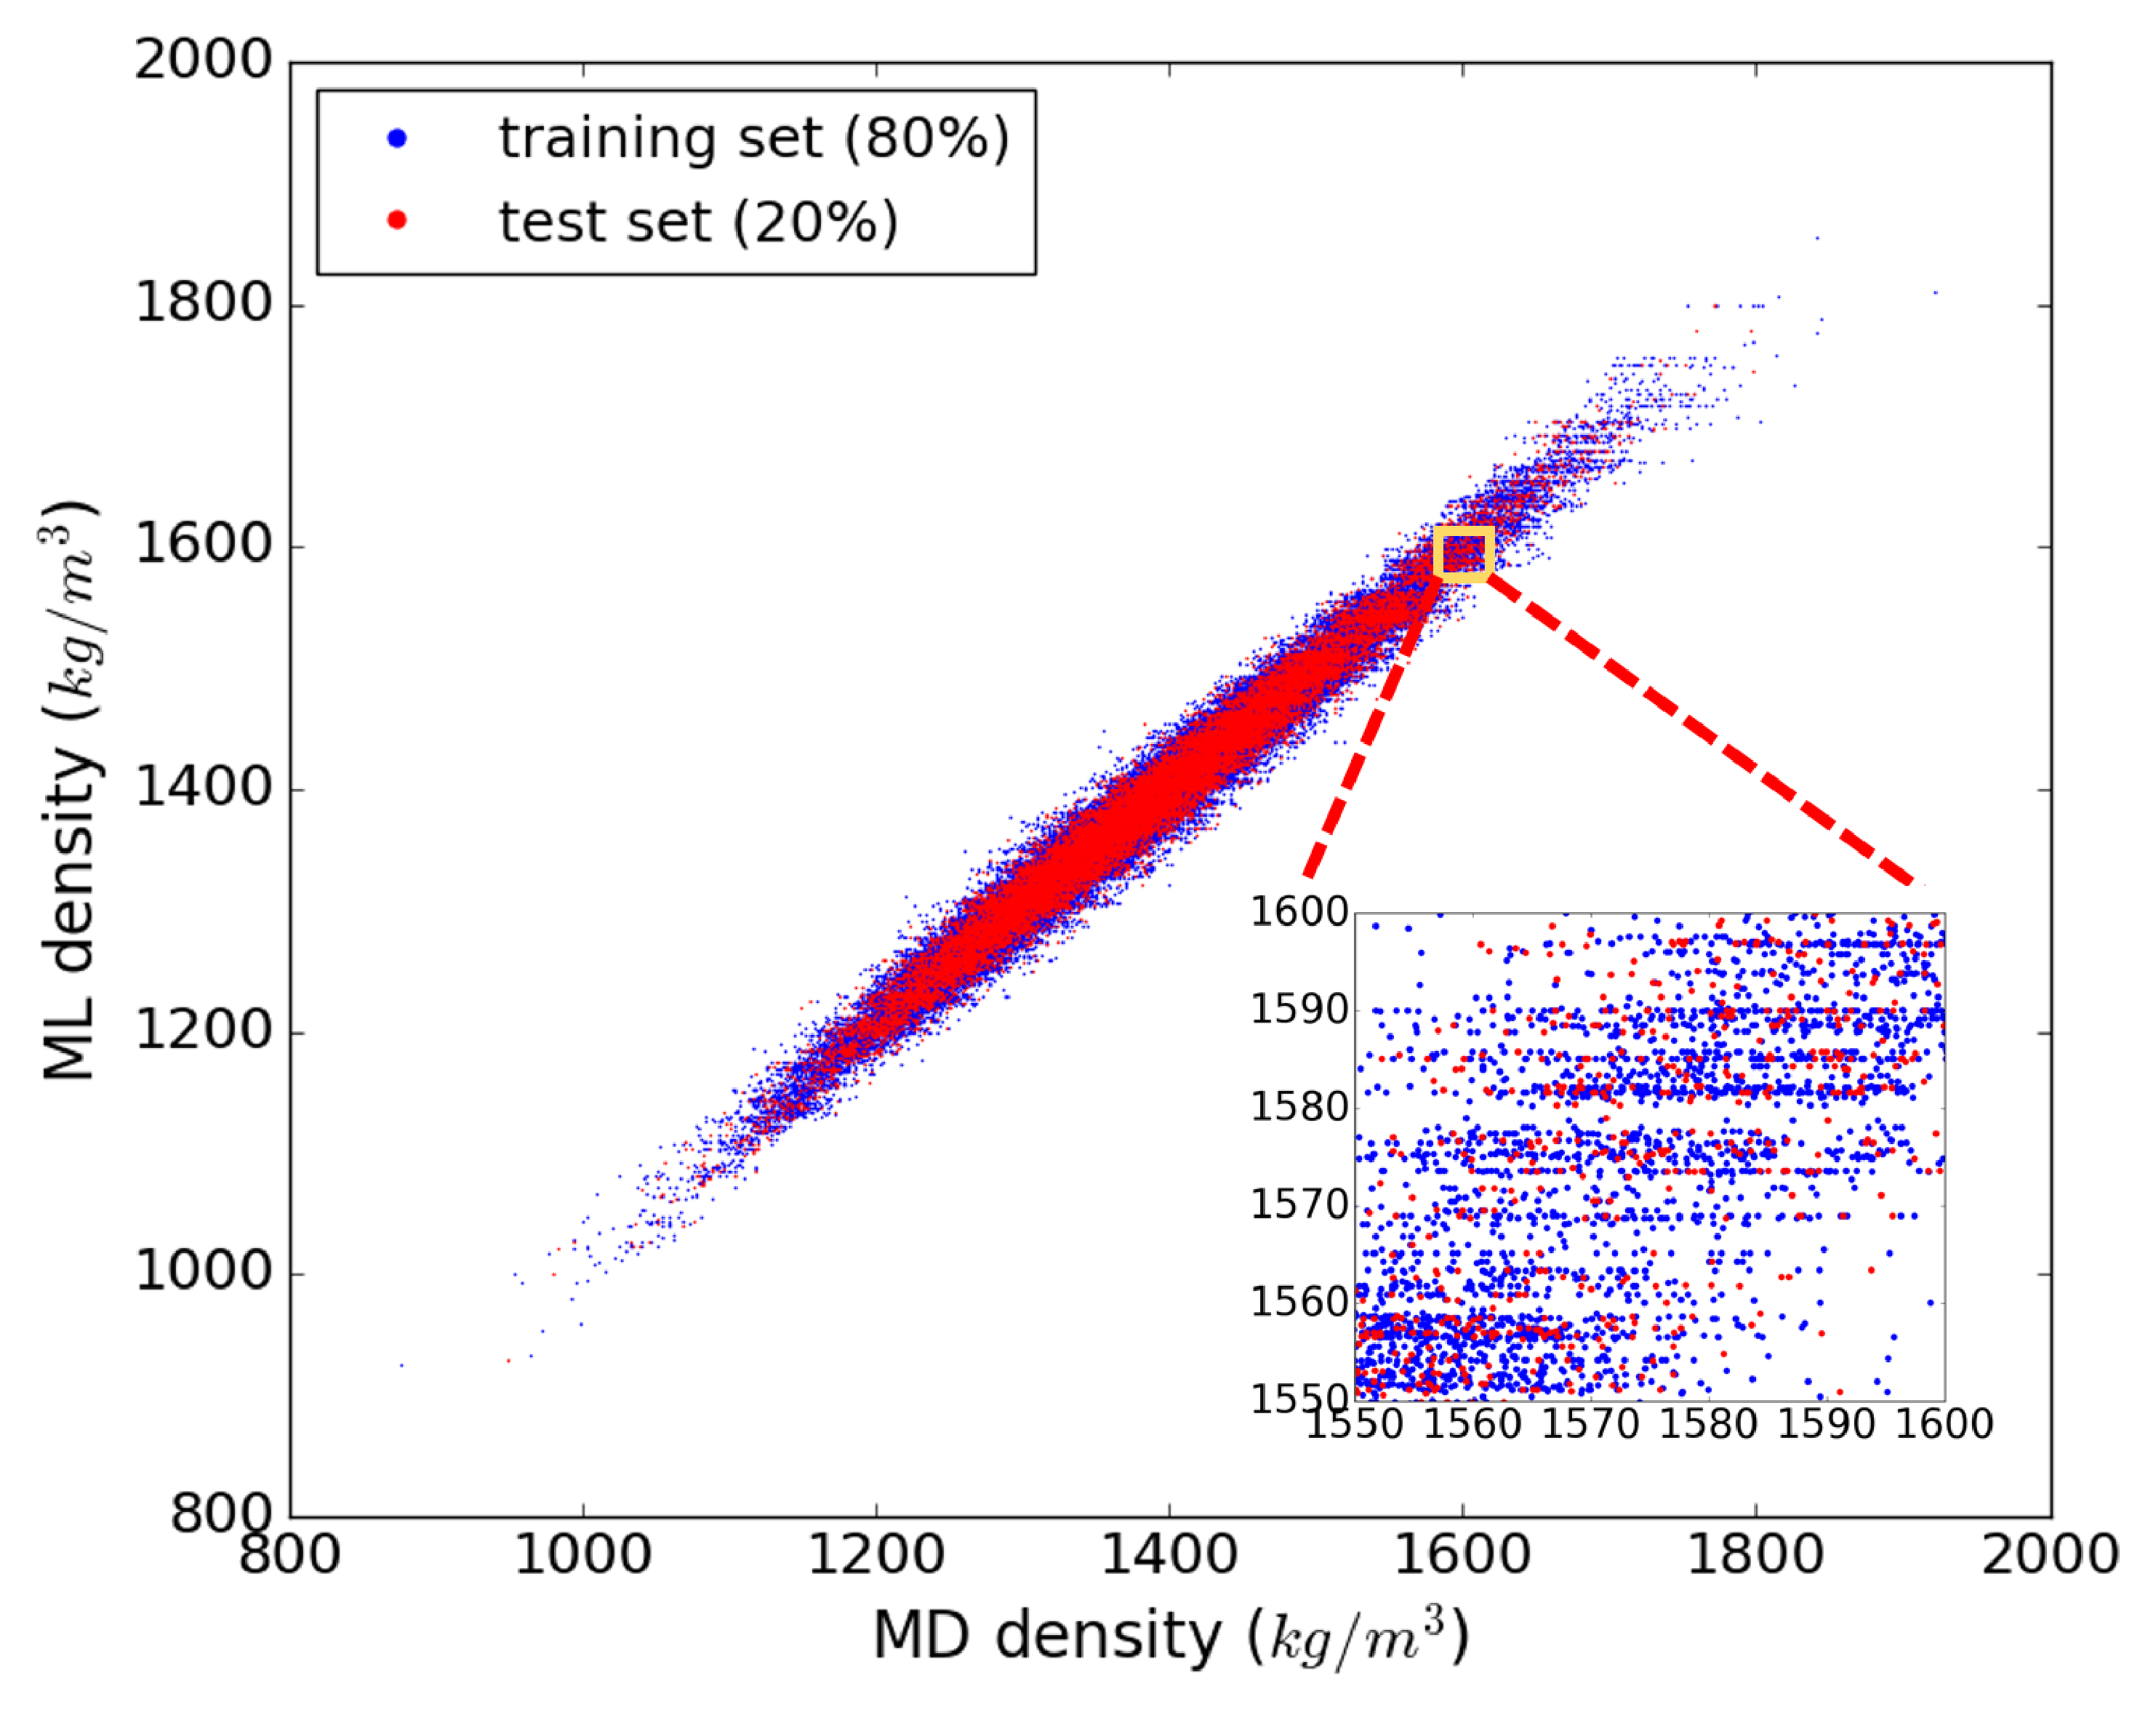
\includegraphics[width=0.744\textwidth]{Chapter-6/Figures/Comparison_MD_NN.eps}
	\caption{Comparing the calculated density (MD) to the predicted density (NN)}
	\label{fig:MD_NN} 
\end{figure} 

Using the developed NN model we were quickly able to calculate the packing density of remaining 1.41 million molecules in the library. The density of these molecules range from 864 $kg/m^3$ to 1645 $kg/m^3$ with an average value of 1261 $kg/m^3$. The distribution of the density of the molecules show a Gaussian distribution with a sigma of 0.084 and variance of 0.007 (see Fig.\ \ref{fig:den_hist}). A low variance in the data indicates that most of the candidates in the library have density values in the range 1200-1600 $kg/m^3$. The number of molecules with density greater than 1600 $kg/m^3$ are very few. Therefore, by a combination of large-scale HTPS and Machine learning, candidates with high density and low density values were identified, which would otherwise not be feasible through empirical studies. Compounds with such extreme packing density values would cater to a specific type of applications, such as, in discovering materials with superior optical properties like refractive index. % the last statement is not necessarily true. We'll have to find another application.

\begin{figure}[htbp] 
	\centering
	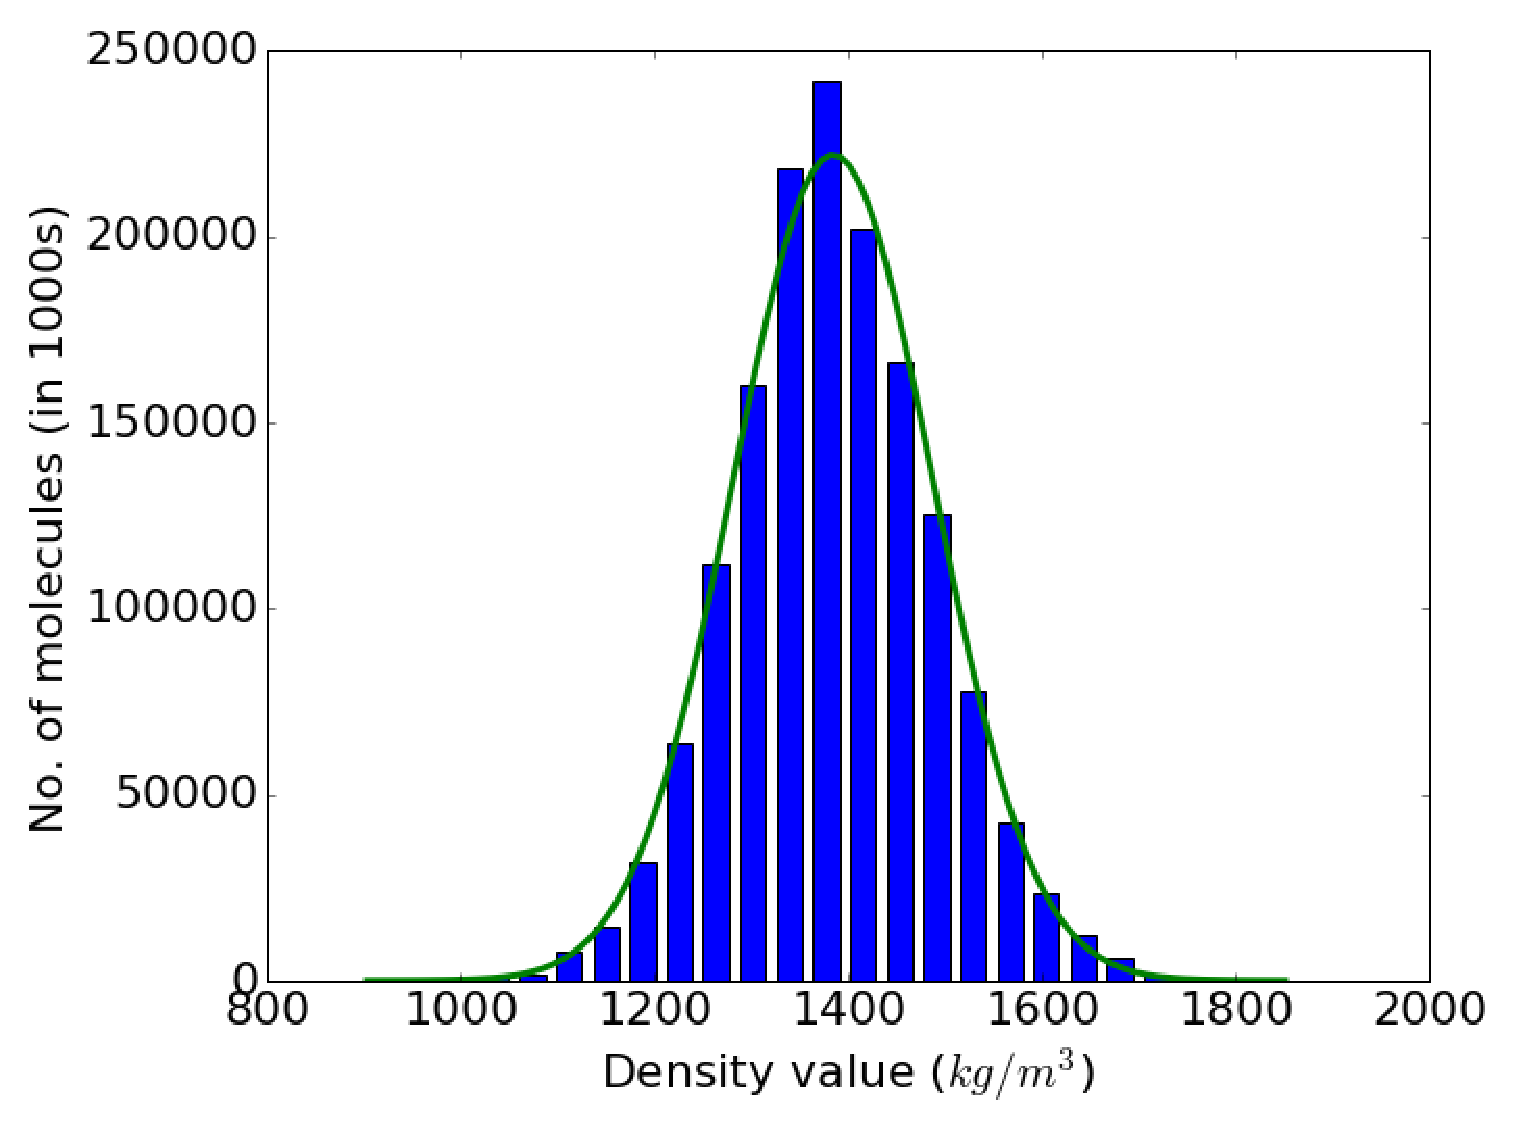
\includegraphics[width=0.744\textwidth]{Chapter-6/Figures/hist.eps}
	\caption{Density vs No. of Molecules} 
	\label{fig:den_hist} 
\end{figure} 

\subsection{Analyzing relationship between molecular structure and density}
\label{subsec:spr}

When considering screening results from a large candidate library, we are not only in a position to assess a large number of compounds, but we can also learn patterns from the data set in its entirety. Thus, in addition to identifying candidates with a targeted density value, we evaluated structure-property relationships by understanding the effect of building blocks on the density of the molecules.

\begin{figure}[htbp] 
	\centering
	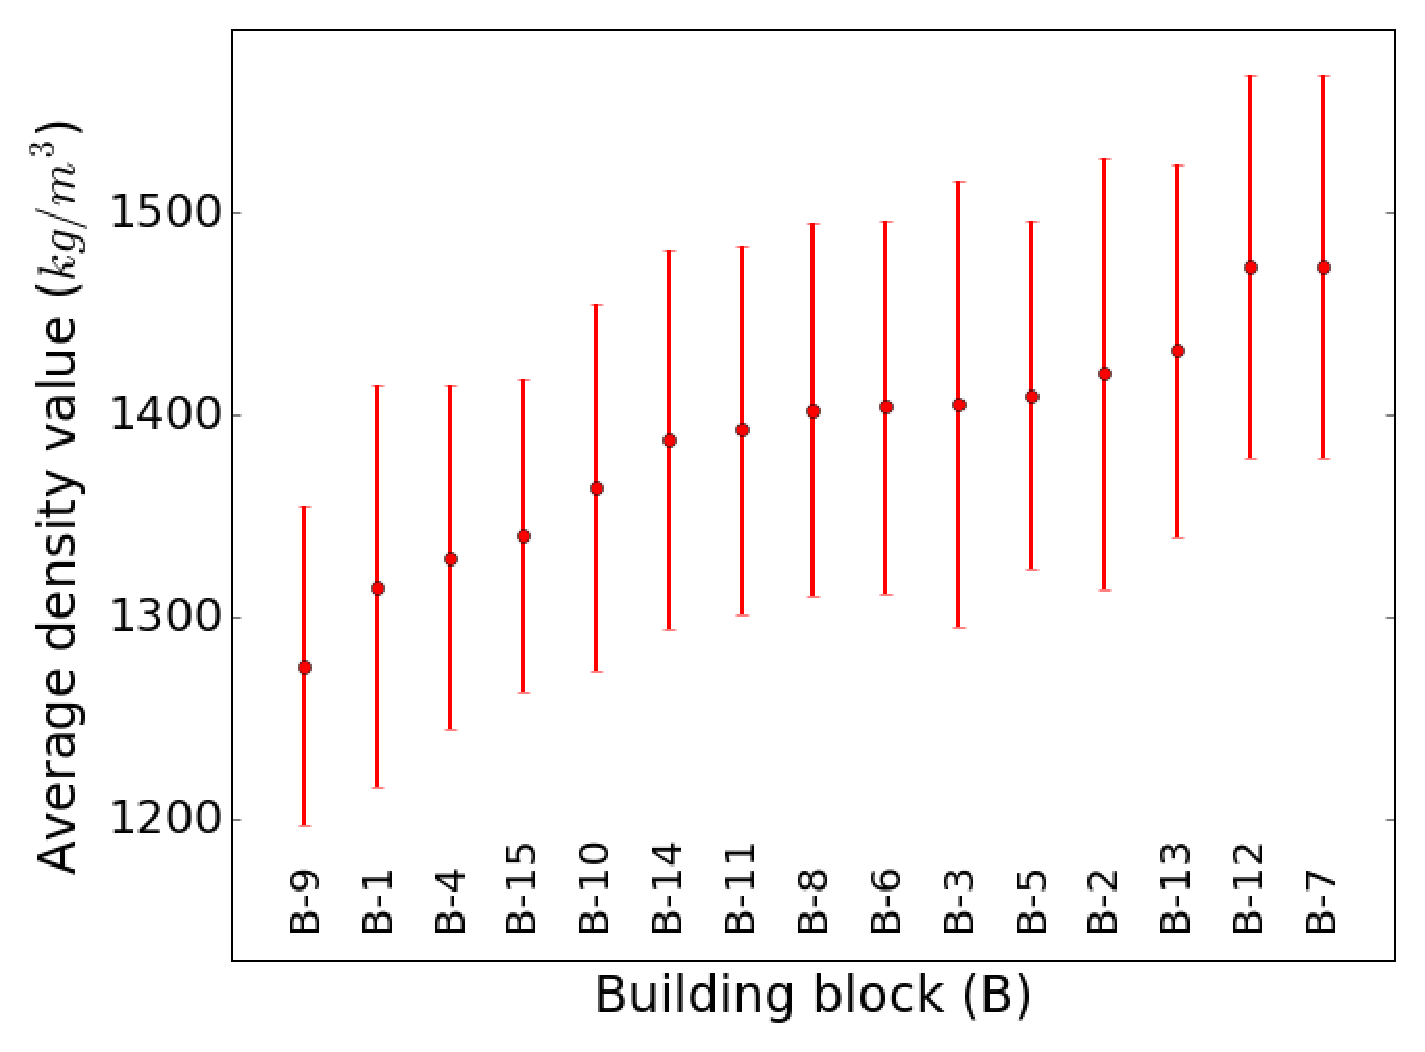
\includegraphics[width=0.744\textwidth]{Chapter-6/Figures/BB_avg_den.eps}
	\caption{Average density for each building blocks}
	\label{fig:bb_avden} 
\end{figure} 

We computed the average density values of all the candidates that contain a particular building block and then ranked the building blocks. The molecules containing building blocks 7 and 12 have the highest average density values, while molecules containing building blocks 1 and 9 have lowest average density values (see Fig.\ \ref{fig:bb_avden}). The average density values shows the cumulative performance of a particular building block, however, it does not present information on the distribution and occurrences of building blocks in a particular subset. Therefore, to generate a more comprehensive structure-property relationship, we evaluated the Z-score of each building block. The Z-score is an indicator of the occurrence of a building block in a subset of the library. The Z-score ($Z_i$) of the building block is calculated by
\[
Z_i=\frac{k-n\frac{K}{N} }{\sigma},\ \sigma=\left [ \frac{nK}{N}\times \left ( \frac{N-K}{N} \right )\times \left ( \frac{N-n}{N-1} \right )\right ]^{\frac{1}{2}}
\]
where $N$ is the total number of molecules, $n$ is the subset of molecules that are considered, $K$ is the number of occurrences of building block $i$ in $N$ molecules and $k$ is the occurrences of building block $i$ in the subset. A large Z-score indicates that a building block appears more frequently in that subset compared to rest of the library. For example, we evaluated the Z-score of building blocks in the 10\% candidates with high density values as shown in the Fig.\ \ref{fig:BB_top_Z}. We observe that building blocks 7 and 12 have high Z-score values, i.e. these building blocks are more prevalent in high density molecules, which is in good agreement with the results from the average density rankings of building blocks shown in Fig.\ \ref{fig:bb_avden}.  

\begin{figure}[htbp] 
	\centering
	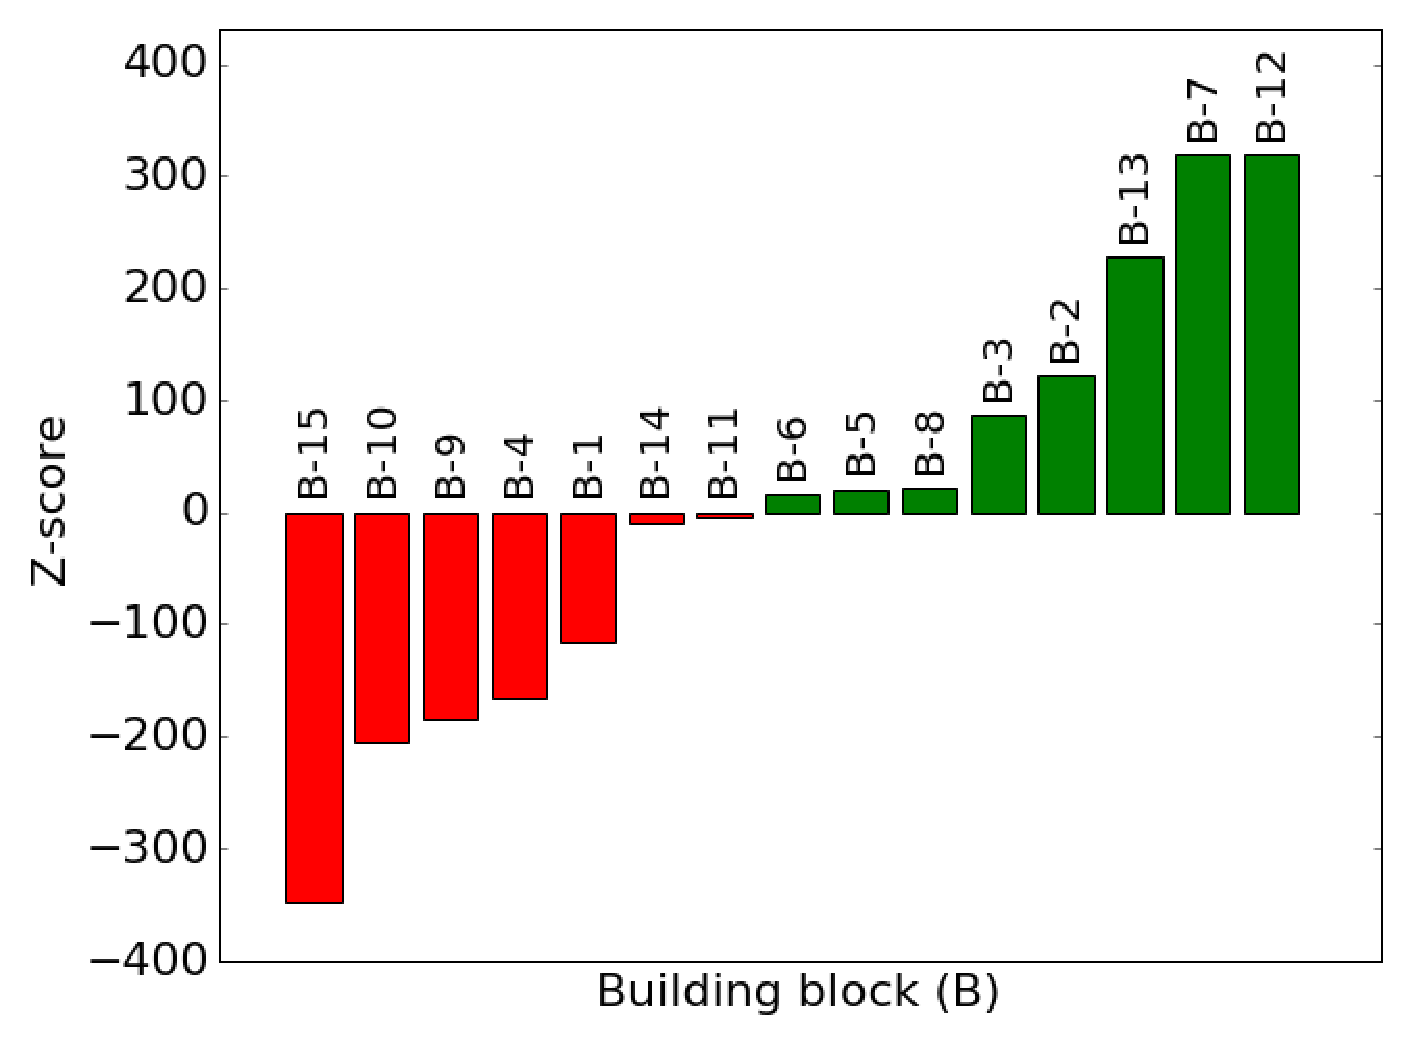
\includegraphics[width=0.744\textwidth]{Chapter-6/Figures/BB_top_Z.eps}
	\caption{Z-score values for each building block}
	\label{fig:BB_top_Z} 
\end{figure} 

\begin{figure*}[htbp] 
	\centering
	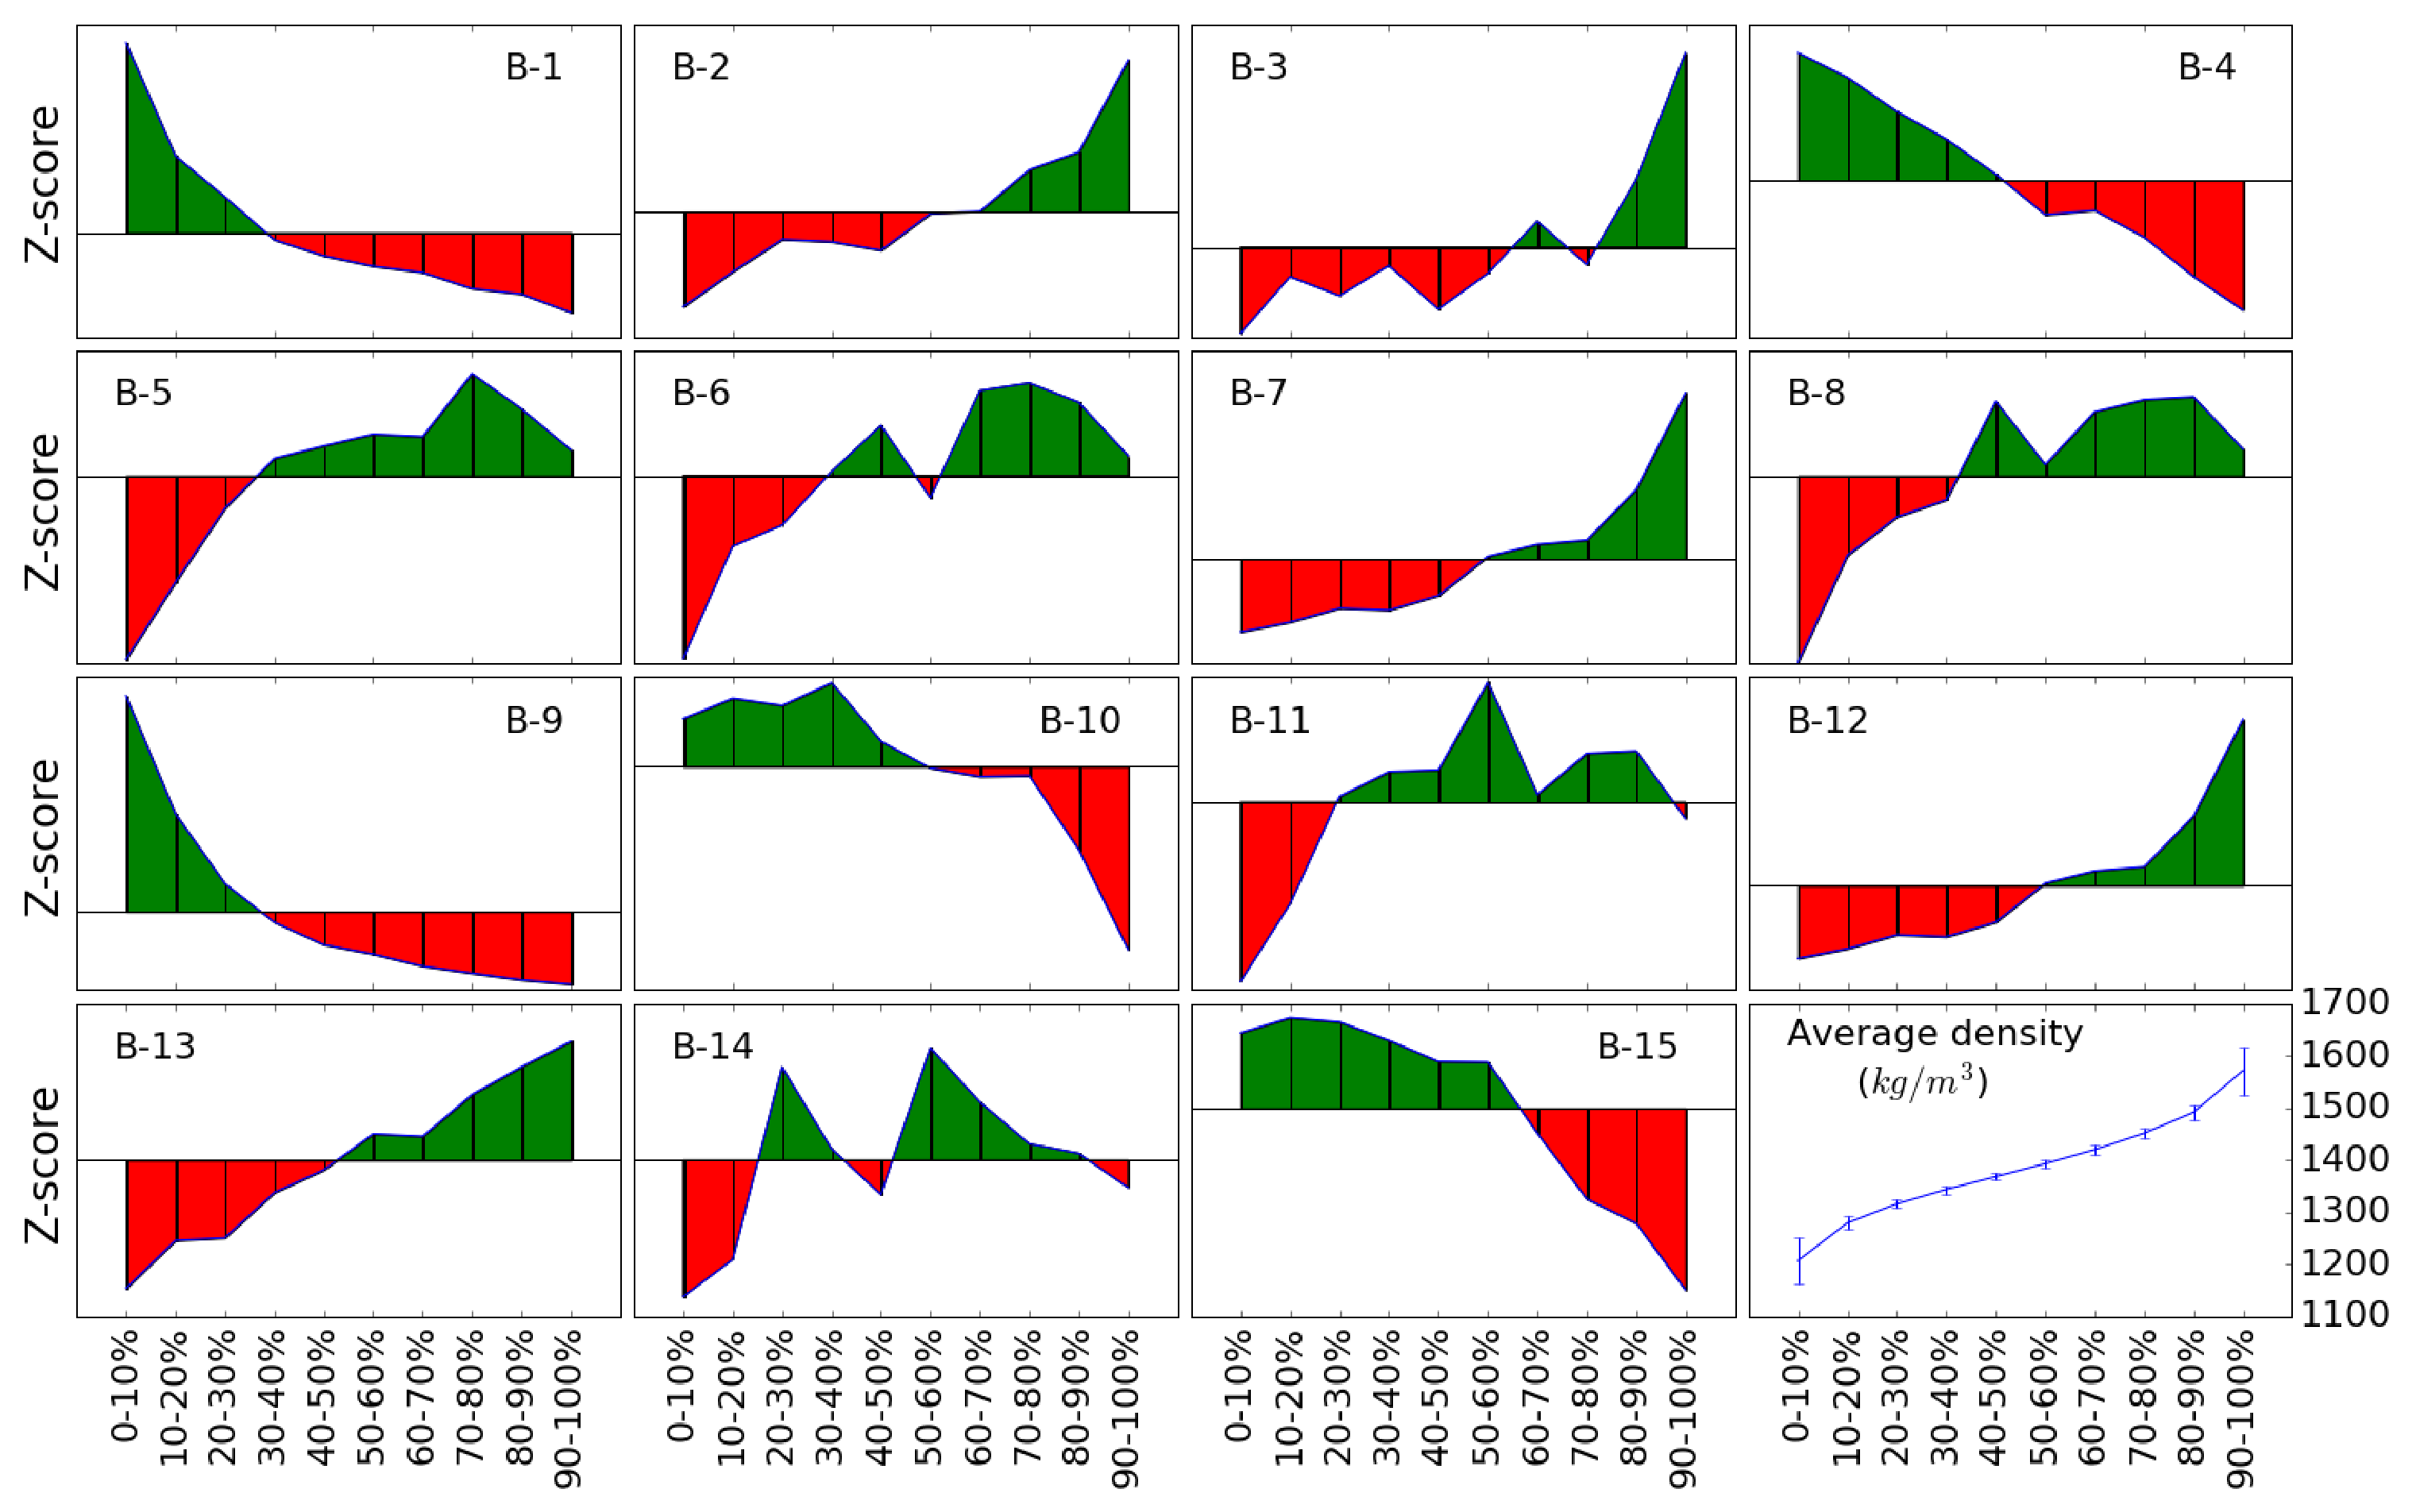
\includegraphics[width=1.0\textwidth]{Chapter-6/Figures/All_BB_Z.eps}
	\caption{Z-score of all the building blocks in the subsets with increasing density values.} 
	\label{fig:BB_all_Z} 
\end{figure*}

In addition to the top 10\% candidates, we use the Z-score analysis method to identify the prevalence of building blocks in the complete spectrum of density values. For this, we sorted the molecular library with increasing density values and then divided into ten equal subsets. Subsequently, the Z-score values of each building block were evaluated in each of these ten subsets and plotted in Fig.\ \ref{fig:BB_all_Z}. The green color in the plot represents a positive Z-score and the red color represents a negative Z-score. Based on the data, we identified certain trends in the performance of individual building blocks. For example, building blocks 2,3,7,12, and 13 would be ideal candidates to develop organic molecules with high density, whereas building blocks 1, 4, 9, 10 and 15 would be better to generate molecules with lower density. %We performed a similar analysis for the polarizability values and subsequently identified molecular targets that can maximize the RI values. 


\subsection{Minimum number of molecules required to learn the model}
\label{subsec:number_of_molecules}

\begin{figure}[htbp] 
	\centering
	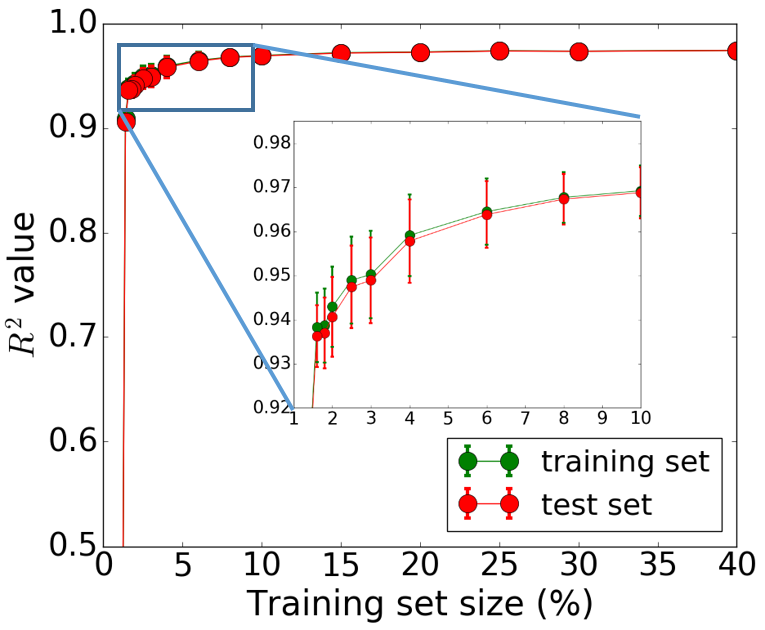
\includegraphics[width=0.744\textwidth]{Chapter-6/Figures/Learning_curve_new.png}
	\caption{Dependence of model accuracy ($R^{2}$) on the training set size.} 
	\label{fig:Learning_curve} 
\end{figure}  

One of the most challenging questions in applying machine learning to learn material properties is what amount of data is required to produce an efficient model. For example, in the current studies we selected 100,000 molecules to learn the density property. However, the question is if we can learn the density from lesser number of molecules. This will allow us to invest less computational resources to perform expensive MD calculations. For this, we varied the size of the training set from 100 to 80,000 molecules (see Fig.\ \ref{fig:Learning_curve}). For all the data sets less than 1800, the model was not able to learn. However, an efficient model can be obtained from using only 2000 molecules. The $R^2$ value keeps increasing until 6000 data sets and then plateaus to a constant value with increasing training size. Thus, we don’t require a large data set of 100,000 molecules to learn the density of organic molecules. We can develop an exceedingly efficient machine learning model just by using 2-6 thousand molecules. This has significant implications on the amount of computational power required to predict the properties of large library of materials. 


\subsection{Descriptors}
\label{subsec:descriptors}

In the inset of Fig.\ \ref{fig:MD_NN}, it can be observed that clusters of the molecules of have similar predicted density value (suggested by the horizontal lines). This might be due the incomplete description of molecules in the selected descriptors. We believe more accurate prediction models can be developed by selecting more comprehensive descriptors such as hashed topological torsion (HTT), Morgan fingerprints, HAP, MACCS, 3D descriptors from Dragon etc. []. In addition to improving features we are also working to implement different deep neural network architecture to improve the learning efficiency. This framework of using machine learning to predict the density of molecules can be extended to learn other material properties. We are currently working on implementing these techniques to predict the optical properties of organic molecules and we will be publishing the results soon.

\section{Conclusions}
\label{sec:conclusions} 

We successfully generated a molecular library of 1.5 million small organic molecules using our in-house molecular library generator. We performed MD simulations on 100,000 compounds to evaluate their packing density values. Using the data from this high-throughput screening, we successfully developed an exceedingly efficient ($R^2$=0.98) neural network model to correlate molecular structural descriptors with their packing density. Using this correlation, we were able to accelerate the density computations of 1.5 million molecules. We mined this huge data and obtained insights into the correlation between the molecular structure and density of materials. Additionally, we evaluated the learning curve for the density prediction to obtain correlation between the model efficiency and size of the data.

We demonstrate that by combining computational modeling and machine learning, we can rapidly and efficiently assess the properties and performance potential of candidate compounds. By combining molecular modeling with virtual high-throughput screening techniques and machine learning, we characterized candidates on a massive scale. We identified design rules as well as high-value building blocks, and structural patterns that correlate with the packing of molecules. These guidelines allow us to target specific molecular motifs and create next generation materials with targeted properties.

